\documentclass{beamer}
\usetheme{CambridgeUS}
\usepackage{enumitem,xcolor}
\setbeamercolor{title}{bg=red!65!black, fg=white}
\setbeamercolor{section in toc}{fg=red!65!black}
\setbeamercolor{section number projected}{bg=red!65!black,fg=white}

\title{High Dynamic Range Imaging}
\author{Semih Dinc \and Ogulcan Seyran}
\date{}

\begin{document}
	\begin{frame}
		\titlepage
		\begin{center}
			Fachbereich Computerwissenschaften Universität Salzburg
		\end{center}
	\end{frame}

	\begin{frame}
		\frametitle{Übersicht}
		\tableofcontents
	\end{frame}

	\section{Allgemein}
	
	\begin{frame}
		\begin{center}
			\Huge Allgemein
		\end{center}
	\end{frame}

	\begin{frame}
		\frametitle{Allgemein}
		\begin{columns}
			\begin{column}{0.7\textwidth}
				\begin{itemize}[label=\textcolor{red!65!black}{\textbullet}]
					\item Erzeugen von Bildern mit hohem Dynamikumfang
					\item Mehrere Methoden zur Erzeugung
					\item High Dynamic Range (HDR): Bilder mit hohem Dynamikumfang
					\item Standard Dynamic Range (SDR): Herkömmliche Bilder
					\item Low Dynamic Range (LDR): Bilder mit niedrigem Dynamikumfang
				\end{itemize}
			\end{column}
			\begin{column}{0.3\textwidth}
					\includegraphics[width=\textwidth]{img/bild1.jpg}
					\tiny www.media.macphun.com
			\end{column}
		\end{columns}
	\end{frame}

	\section{Anwendungsgebiete}
	
	\begin{frame}
		\begin{center}
			\Huge Anwendungsgebiete
		\end{center}
	\end{frame}

	\begin{frame}
		\frametitle{Anwendungsgebiete}
		\begin{columns}
			\begin{column}{0.5\textwidth}
			\textbf{Computergrafiken}\\
			\small Berechnen von kontrastreichen 3D Szenen\\
			\vspace{5mm}
			\textbf{Digitalfotografie}\\
			\small Detailreiche / Realitätsnahe Fotos \\
			\vspace{5mm}
			\textbf{Virtuelle Realität}\\
			\small Anpassung an virtuelle Umgebung und individuelle Komprimierung \\
			\vspace{5mm}
			\textbf{Überwachungssysteme}\\
			\small Extreme Lichtverhältnisse
			\end{column}
			\begin{column}{0.5\textwidth}
			\textbf{Maschinelles Sehen}\\
			\small Erfassen von Bilddetails für maschinelle Verarbeitung \\
			\vspace{5mm} 
			\textbf{Medizin}\\
			\small Kleine Bildsensoren und geringe Helligkeit \\
			\vspace{5mm} 
			\textbf{Architektur}\\
			\small Abbild von Lichtverteilungen in Szenen
			\end{column}
		\end{columns}
	\end{frame}

	\section{Dynamikumfang}
	
	\begin{frame}
		\begin{center}
			\Huge Dynamikumfang
		\end{center}
	\end{frame}

	\begin{frame}
		\frametitle{Dynamikumfang}
		\begin{itemize}[label=\textcolor{red!65!black}{\textbullet}]
			\item Verhältnis zwischen der hellsten und dunkelsten Stelle
			\item Je größer der Dynamikumfang desto mehr Helligkeitsabstufungen sind verfügbar
			\item Niedriger Dynamikumfang sorgt für detailarme Bilder
			\item Begrenzter Dynamikumfang in Kameras
			\item Menschliches Auge um vielfaches höheren Dynamikumfang
			\item Informationsverlust bei dunklen und hellen Stellen
			\item Lichtstopps bestimmen Dynamikumfang
			\begin{center}
				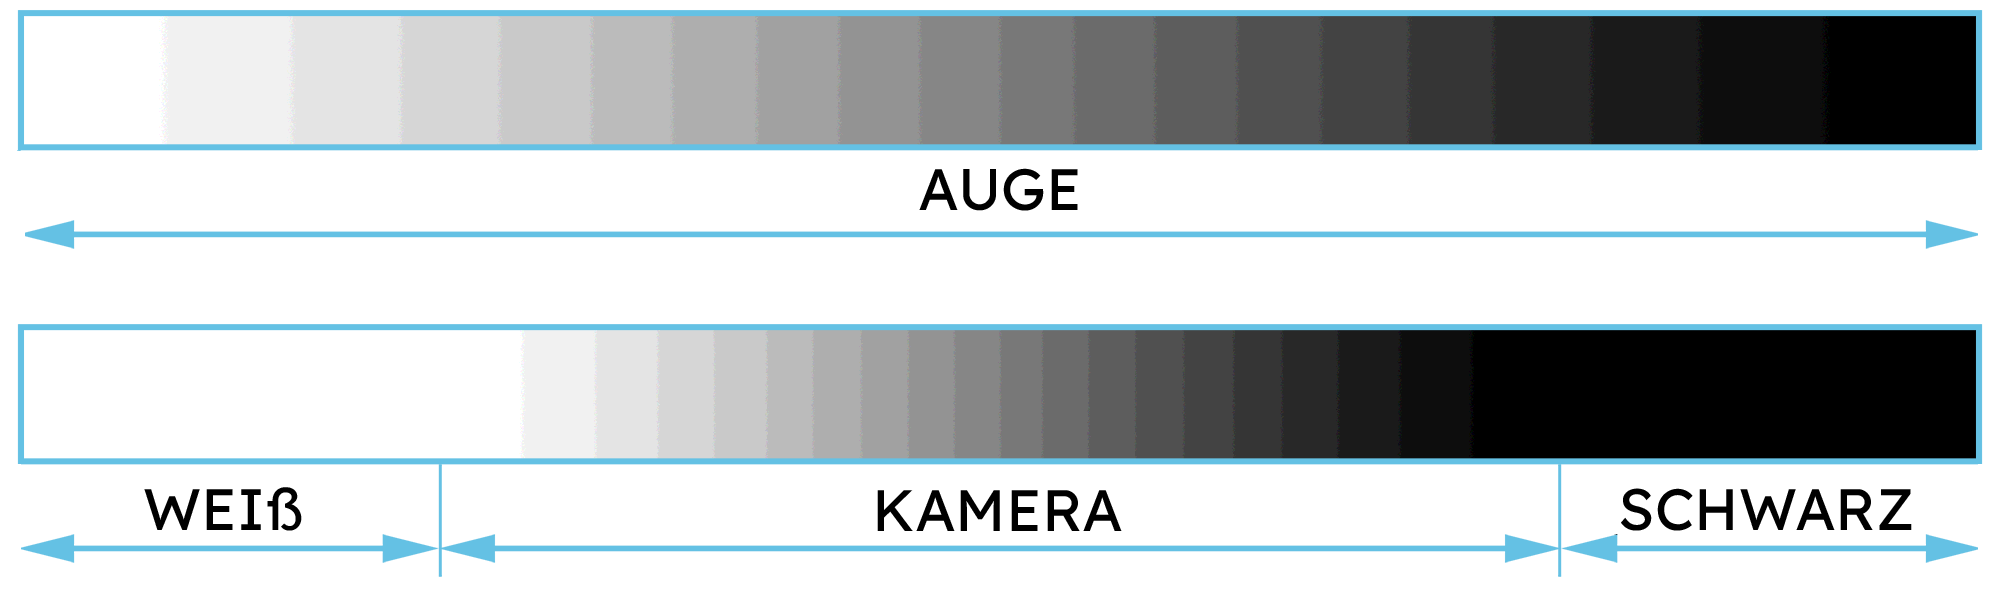
\includegraphics[scale=0.4]{img/Bild2.png}
				\tiny www.littleowlpictures.de
			\end{center}
		\end{itemize}
	\end{frame}
	
	\begin{frame}
	\frametitle{Lichtstopp}
	\begin{columns}
		\begin{column}{0.55\textwidth}
			\textbf{Besagt wieviel Licht durchkommt} \\
			\small \hspace{2mm} +1 F-Stop halbiert die Menge an Licht\\
			\small \hspace{2mm} -1 F-Stop verdoppelt die Menge an Licht\\
			\vspace{5mm}
			\textbf{Dynamikumfang berechnen} \\
			\indent
			\small \hspace{2mm} f/4\\
			\small \hspace{2mm} 2$^{4}$ = 16\\
			\small \hspace{2mm} Dynamikumfang 1 : 16\\
			\vspace{5mm}
			\textbf{Kamera} \\
			\small \hspace{2mm} f/17 -1 : 130 000\\
			\vspace{5mm}
			\textbf{Menschliches Auge} \\
			\small \hspace{2mm} + f/20 - 1 : 1 000 000\\
		\end{column}
		\begin{column}{0.45\textwidth}
			\includegraphics[scale=0.35]{img/bild3.png}
			\tiny www.en.wikipedia.org/wiki/User:Cbuckley
		\end{column}
	\end{columns}
	\end{frame}

	\begin{frame}
	\frametitle{Vergleich}
	\begin{columns}
		\begin{column}{0.5\textwidth}
			\begin{center}
				\textbf{Niedriger Dynamikumfang} \\
				\small Informationsverlust und Verfälschung von Farben in zu hellen und dunklen Bereichen \\
				\includegraphics[scale=0.35]{img/bild4.jpg}
				\tiny www.ai.googleblog.com
			\end{center}
		\end{column}
		\begin{column}{0.5\textwidth}
			\begin{center}
				\textbf{Hoher Dynamikumfang} \\
				\small Informationen erhalten, Strukturen erkennbar, Farben realitätsnahe dargestellt \\
				\includegraphics[scale=0.35]{img/bild5.jpg}
				\tiny www.ai.googleblog.com
			\end{center}
		\end{column}
	\end{columns}
	\end{frame}
	
	\section{Dynamikkompression}
	\begin{frame}
		\begin{center}
			\Huge Dynamikkompression
		\end{center}
	\end{frame}

	\begin{frame}
	\frametitle{Dynamikkompression}
	\begin{columns}
		\begin{column}{0.5\textwidth}
			\begin{itemize}[label=\textcolor{red!65!black}{\textbullet}]
				\item Komprimierung des Dynamikumfangs um HDR Inhalte auf herkömmlichen Endgeräten darzustellen
				\item Helligkeitsbereich vom Bild muss so komprimiert werden, dass es in den Helligkeitsbereich des Endgeräts passt
				\item Großes Spektrum an Kontrast und Dynamik geht verloren
				\item Mit guter Kompression sehen HDR Inhalte auch auf SDR Bildschirmen gut aus
			\end{itemize}
		\end{column}
		\begin{column}{0.5\textwidth}
			\includegraphics[scale=0.43]{img/bild6.png}
			\tiny www.redway3d.com
		\end{column}
	\end{columns}
	\end{frame}

	\begin{frame}
	\frametitle{Dynamikkompression bei Endgeräten}
	\begin{center}
		\includegraphics[scale=0.45]{img/bild7.png}
		\tiny www.terms.tta.or.kr
	\end{center}
	\end{frame}

	\section{HDR Endgeräte}
	\begin{frame}
		\begin{center}
			\Huge HDR Endgeräte
		\end{center}
	\end{frame}
	\begin{frame}
	\frametitle{Allgemein}
	\begin{itemize}[label=\textcolor{red!65!black}{\textbullet}]
		\item In der Lage viel höhere Dynamikbereiche zu repräsentieren
		\item Um ein vielfaches hellere Darstellung (Nits)
		\item Je heller der Bildschirm desto mehr Dynamik kann er wiedergeben
	\end{itemize}
	\end{frame}

	\begin{frame}
	\frametitle{Darstellungsspektrum}
	\begin{center}
		\includegraphics[scale=0.45]{img/bild8.png}
		\tiny www.terms.tta.or.kr
	\end{center}
	\end{frame}

	\section{Methoden}
	
	\begin{frame}
		\begin{center}
			\Huge Methoden
		\end{center}
	\end{frame}

	\begin{frame}
	\frametitle{HDR Kamera}
	\begin{itemize}[label=\textcolor{red!65!black}{\textbullet}]
		\item Leistungsfähige Sensoren
		\item Einsatz unter extremen Lichtbedingungen
		\item Nutzung spezieller Verfahren und Algorithmen
	\end{itemize}
	\vspace{5mm}
	\hspace{7mm} \textbf{HDRC (High Dynamic Range CMOS)} \\
	\small \hspace{9mm} Weiterentwicklung des CMOS Sensor \\
	\small \hspace{9mm} Ähnelt Empfindlichkeit des menschlichen Auges
	\end{frame}

	\begin{frame}
	\frametitle{Belichtungsreihen}
	\begin{columns}
		\begin{column}{0.55\textwidth}
			\begin{itemize}[label=\textcolor{red!65!black}{\textbullet}]
				\item Erstellen von mehreren Bildern mit unterschiedlichen Belichtungsstufen	
				\item Zusammenfügen automatisch in Kamera oder nachträglich in Software
			\end{itemize}
		\end{column}
		\begin{column}{0.45\textwidth}
			\includegraphics[scale=0.5]{img/bild9.jpg}
			\tiny www.traumflieger.de
		\end{column}
	\end{columns}
	\end{frame}

	\begin{frame}
	\frametitle{Software}
	\textbf{Belichtungsreihen zusammenfügen in Software}
	\begin{itemize}[label=\textcolor{red!65!black}{\textbullet}]
		\item Gratis Software verfügbar
		\item Automatische Zusammenführung von Belichtungsreihen
		\item Farbeinstellungen
		\item Dynamikkompresion möglich
		\item Beispiel anhand easyHDR
	\end{itemize}
	\end{frame}

	\begin{frame}
	\frametitle{Beispiel Belichtungsreihe}
	\begin{columns}
		\begin{column}{0.33\textwidth}
			\begin{center}
				\textbf{Unterbelichtet}\\
				\vspace{5mm}
				\includegraphics[scale=0.4]{img/bild10.jpg}
				\tiny www.hdrsoft.com
			\end{center}
		\end{column}
		\begin{column}{0.33\textwidth}
			\begin{center}
				\textbf{Normal belichtet} \\
				\vspace{5mm}
				\includegraphics[scale=0.4]{img/bild11.jpg}
				\tiny www.hdrsoft.com
			\end{center}
		\end{column}
		\begin{column}{0.33\textwidth}
			\begin{center}
			\textbf{Überbelichtet} \\ 
			\vspace{5mm}
			\includegraphics[scale=0.4]{img/bild12.jpg}
			\tiny www.hdrsoft.com
			\end{center}
		\end{column}
	\end{columns}
	\end{frame}

	\begin{frame}
	\frametitle{Resultat}
	\begin{columns}
		\begin{column}{0.5\textwidth}
			\begin{center}
				\textbf{Normal Belichtet} \\ 
				\vspace{5mm}
				\includegraphics[scale=0.42]{img/bild13.jpg}
				\tiny www.hdrsoft.com
			\end{center}
		\end{column}
		\begin{column}{0.5\textwidth}
			\begin{center}
				\textbf{Resultat (HDR)} \\ 
				\vspace{5mm}
				\includegraphics[scale=0.42]{img/bild14.png}
				\tiny www.hdrsoft.com
			\end{center}
		\end{column}
	\end{columns}
	\end{frame}

	\begin{frame}
	\frametitle{HDR Rendering}
	\begin{columns}
		\begin{column}{0.55\textwidth}
			\begin{itemize}[label=\textcolor{red!65!black}{\textbullet}]
				\item Rendering unter Berücksichtigung der in der Natur vorkommenden großen Helligkeitsschwankungen	
				\item Darstellung starker Kontraste ohne übermäßigen Detailverlust	
			\end{itemize}
			\vspace{5mm}
			\hspace{7mm} \textbf{Image-Based Lighting} \\
			\vspace{3mm}
			\hspace*{9mm}
			\begin{minipage}{0.8\textwidth}
				\small  Szene wird von einem HDR-Bild umhüllt und beleuchtet. \\
				\small  Sieht so aus als wären die Künstlichen Objekte in einer natürlichen Umgebung. \\
			\end{minipage}

		\end{column}
		\begin{column}{0.45\textwidth}
				\includegraphics[scale=0.37]{img/bild15.jpg}
				\tiny www.flickr.com : Miles Bader
		\end{column}
	\end{columns}
	\end{frame}

	\section{Formate}
	\begin{frame}
		\begin{center}
			\Huge Formate
		\end{center}
	\end{frame}
	\begin{frame}
	\frametitle{Verlustbehaftete und Verlustfreie Kompression}
	\begin{columns}
		\begin{column}{0.5\textwidth}
			\textbf{Verlustbehaftete Kompression}
			\begin{itemize}[label=\textcolor{red!65!black}{\textbullet}]
				\item Meist für Video Material
				\item Wiederhergestelltes Bild ist eine ähnliche Wiedergabe des Originales, aber kein Duplikat
				\item Komprimiert eher die Bereiche, die vom menschlichen Auge schlechter wahrgenommen werden
			\end{itemize}
		\end{column}
		\begin{column}{0.5\textwidth}
			\textbf{Verlustfreie Kompression}
			\begin{itemize}[label=\textcolor{red!65!black}{\textbullet}]
				\item Wiederherstellung aller vorhandenen Daten vom Originalbild
				\item Eignet sich für Bilder, die große Mengen an wiederholt enthaltenen Informationen beinhaltet
				\item z.B.: Blauer Himmel
				\item Bekannte Verfahren z.B.: Huffman-Kodierung
			\end{itemize}
		\end{column}
	\end{columns}
	\end{frame}

	\begin{frame}
	\frametitle{Verbreitete Formate}
		Unterscheiden sich Hauptsächlich in Kodierung, Kompression und Farb- und Helligkeitswerten \\
		Derzeit gibt es zwei große HDR-Formate in der Medienbranche \\
		\vspace{5mm}
		\textbf{HDR10}
		\begin{itemize}[label=\textcolor{red!65!black}{\textbullet}]
			\item standartisiertes Format
			\item Farbtiefe 10 Bit
			\item Farb- und Helligkeitswerte in einem vordefinierten Bereich
		\end{itemize}
			\textbf{Dolby-Vision}
		\begin{itemize}[label=\textcolor{red!65!black}{\textbullet}]
			\item Farbtiefe 12 Bit, abwärtskompatibel
			\item Farb- und Helligkeitswerte basierend auf das jeweilige Profil des Gerätes
		\end{itemize}
	\end{frame}

	\begin{frame}[allowframebreaks]
		\frametitle{Quellenverzeichnis}
			\nocite{*}
			\bibliographystyle{plain}
			\bibliography{kombinierte_referenzen}
	\end{frame}

\end{document}